%%%%%%%%%%%%%%%%%%%%%%%%%%%%%%%%%%%%%%%%%%%%%%%%%%%%%%%%%%%%%%%%%%%%%%%%%%%%%%%%%%%%%%%%%%%%%%%%%%%%%%%%%%%%%%

\begin{exercise}{Diagramme $E$-pH du Zirconium}{0}{Sup}
{Diagramme E-pH}{bermu}

On demande dans cet exercice de tracer le diagramme potentiel-pH du zirconium en solution aqueuse
et de l’utiliser pour discuter de la stabilité du métal au contact de l’eau.




\paragraph{Données :}
\begin{itemize}
    \item Concentration de tracé $c_\text{tra} = \SI{1.0e-6}{mol.L{-1}}\qquad$ (corrosion)

    \item $E^\circ(\mathrm{Zr^{4+_{(aq)}}/Zr_{(s)}}) = \SI{-1,44}{V}$

    \item $\text{p}K_\text{s}(\mathrm{ZrO_{2(s)}/Zr^{4+}_{(aq)}}) = 55,1\qquad$ (en milieu basique)

    \item $\text{p}K_\text{d}(\mathrm{(HZrO_3)^-_{(aq)}/ZrO_{2(s)}}) = 4,8\qquad$ (en milieu basique)

\end{itemize}

\end{exercise}

\begin{solution}

~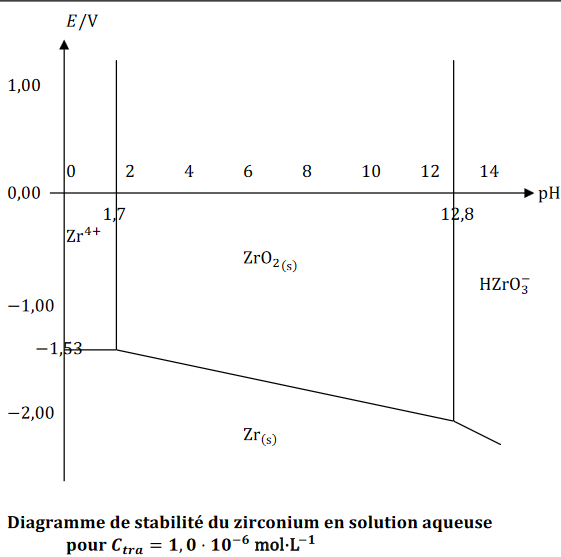
\includegraphics[]{chimie/E-pH/zirco.png}

\end{solution}